\documentclass[a4paper]{article}

%--------------------------------------------------------------------------
\usepackage[a4paper, total={6in, 9in}]{geometry}
\usepackage{amsmath}
\usepackage{booktabs}
\usepackage{caption}
\usepackage{graphicx}
\usepackage{float}
\usepackage{inconsolata}
\usepackage{listings}
\usepackage{xcolor}
\usepackage{siunitx}
\usepackage[most]{tcolorbox}
\usepackage{etoolbox}

\makeatletter
\patchcmd{\l@section}
{\hfil}
{\leaders\hbox{\normalfont$\m@th\mkern \@dotsep mu\hbox{.}\mkern \@dotsep mu$}\hfill}
{}{}
\makeatother

%--------------------------------------------------------------------------
\graphicspath{{./fig/}}

%--------------------------------------------------------------------------


\definecolor{mGreen}{rgb}{0,0.6,0}
\definecolor{mGray}{rgb}{0.5,0.5,0.5}
\definecolor{mPurple}{rgb}{0.58,0,0.82}
\definecolor{backgroundColour}{rgb}{0.95,0.95,0.92}

\lstdefinestyle{CStyle}{
	backgroundcolor=\color{backgroundColour},   
	commentstyle=\color{mGreen},
	keywordstyle=\color{magenta},
	numberstyle=\tiny\color{mGray},
	stringstyle=\color{mPurple},
	basicstyle=\footnotesize,
	breakatwhitespace=false,         
	breaklines=true,                 
	captionpos=b,                    
	keepspaces=true,                 
	numbers=left,                    
	numbersep=5pt,                  
	showspaces=false,                
	showstringspaces=false,
	showtabs=false,                  
	tabsize=2,
	language=C
}

\setlength\parindent{0pt}

%--------------------------------------------------------------------------
\begin{document}
\title{HIT332: Embedded and Mobile Systems\\ Practical 4 Notes}
\author{Shane Reynolds}
\maketitle

\tableofcontents

%--------------------------------------------------------------------------
\section{Introduction \& Background}

The intention behind this brief set of notes is to provide guidance on how well the practicals and projects for HIT332: Embedded and Mobile Systems achieve their intended outcomes. There are 5 practicals in total, and 3 projects. This set of notes will cover Practical 4. The practicals (and projects) make use of a development board created by Damien Hill and Ben Saunders of Charles Darwin University. The main component of the board is the Atmel ATmega1281 16au 16MHz, 8-bit microcontroller. The development board can be seen in Figure 1.

\begin{figure}[h]
	\centering
	\frame{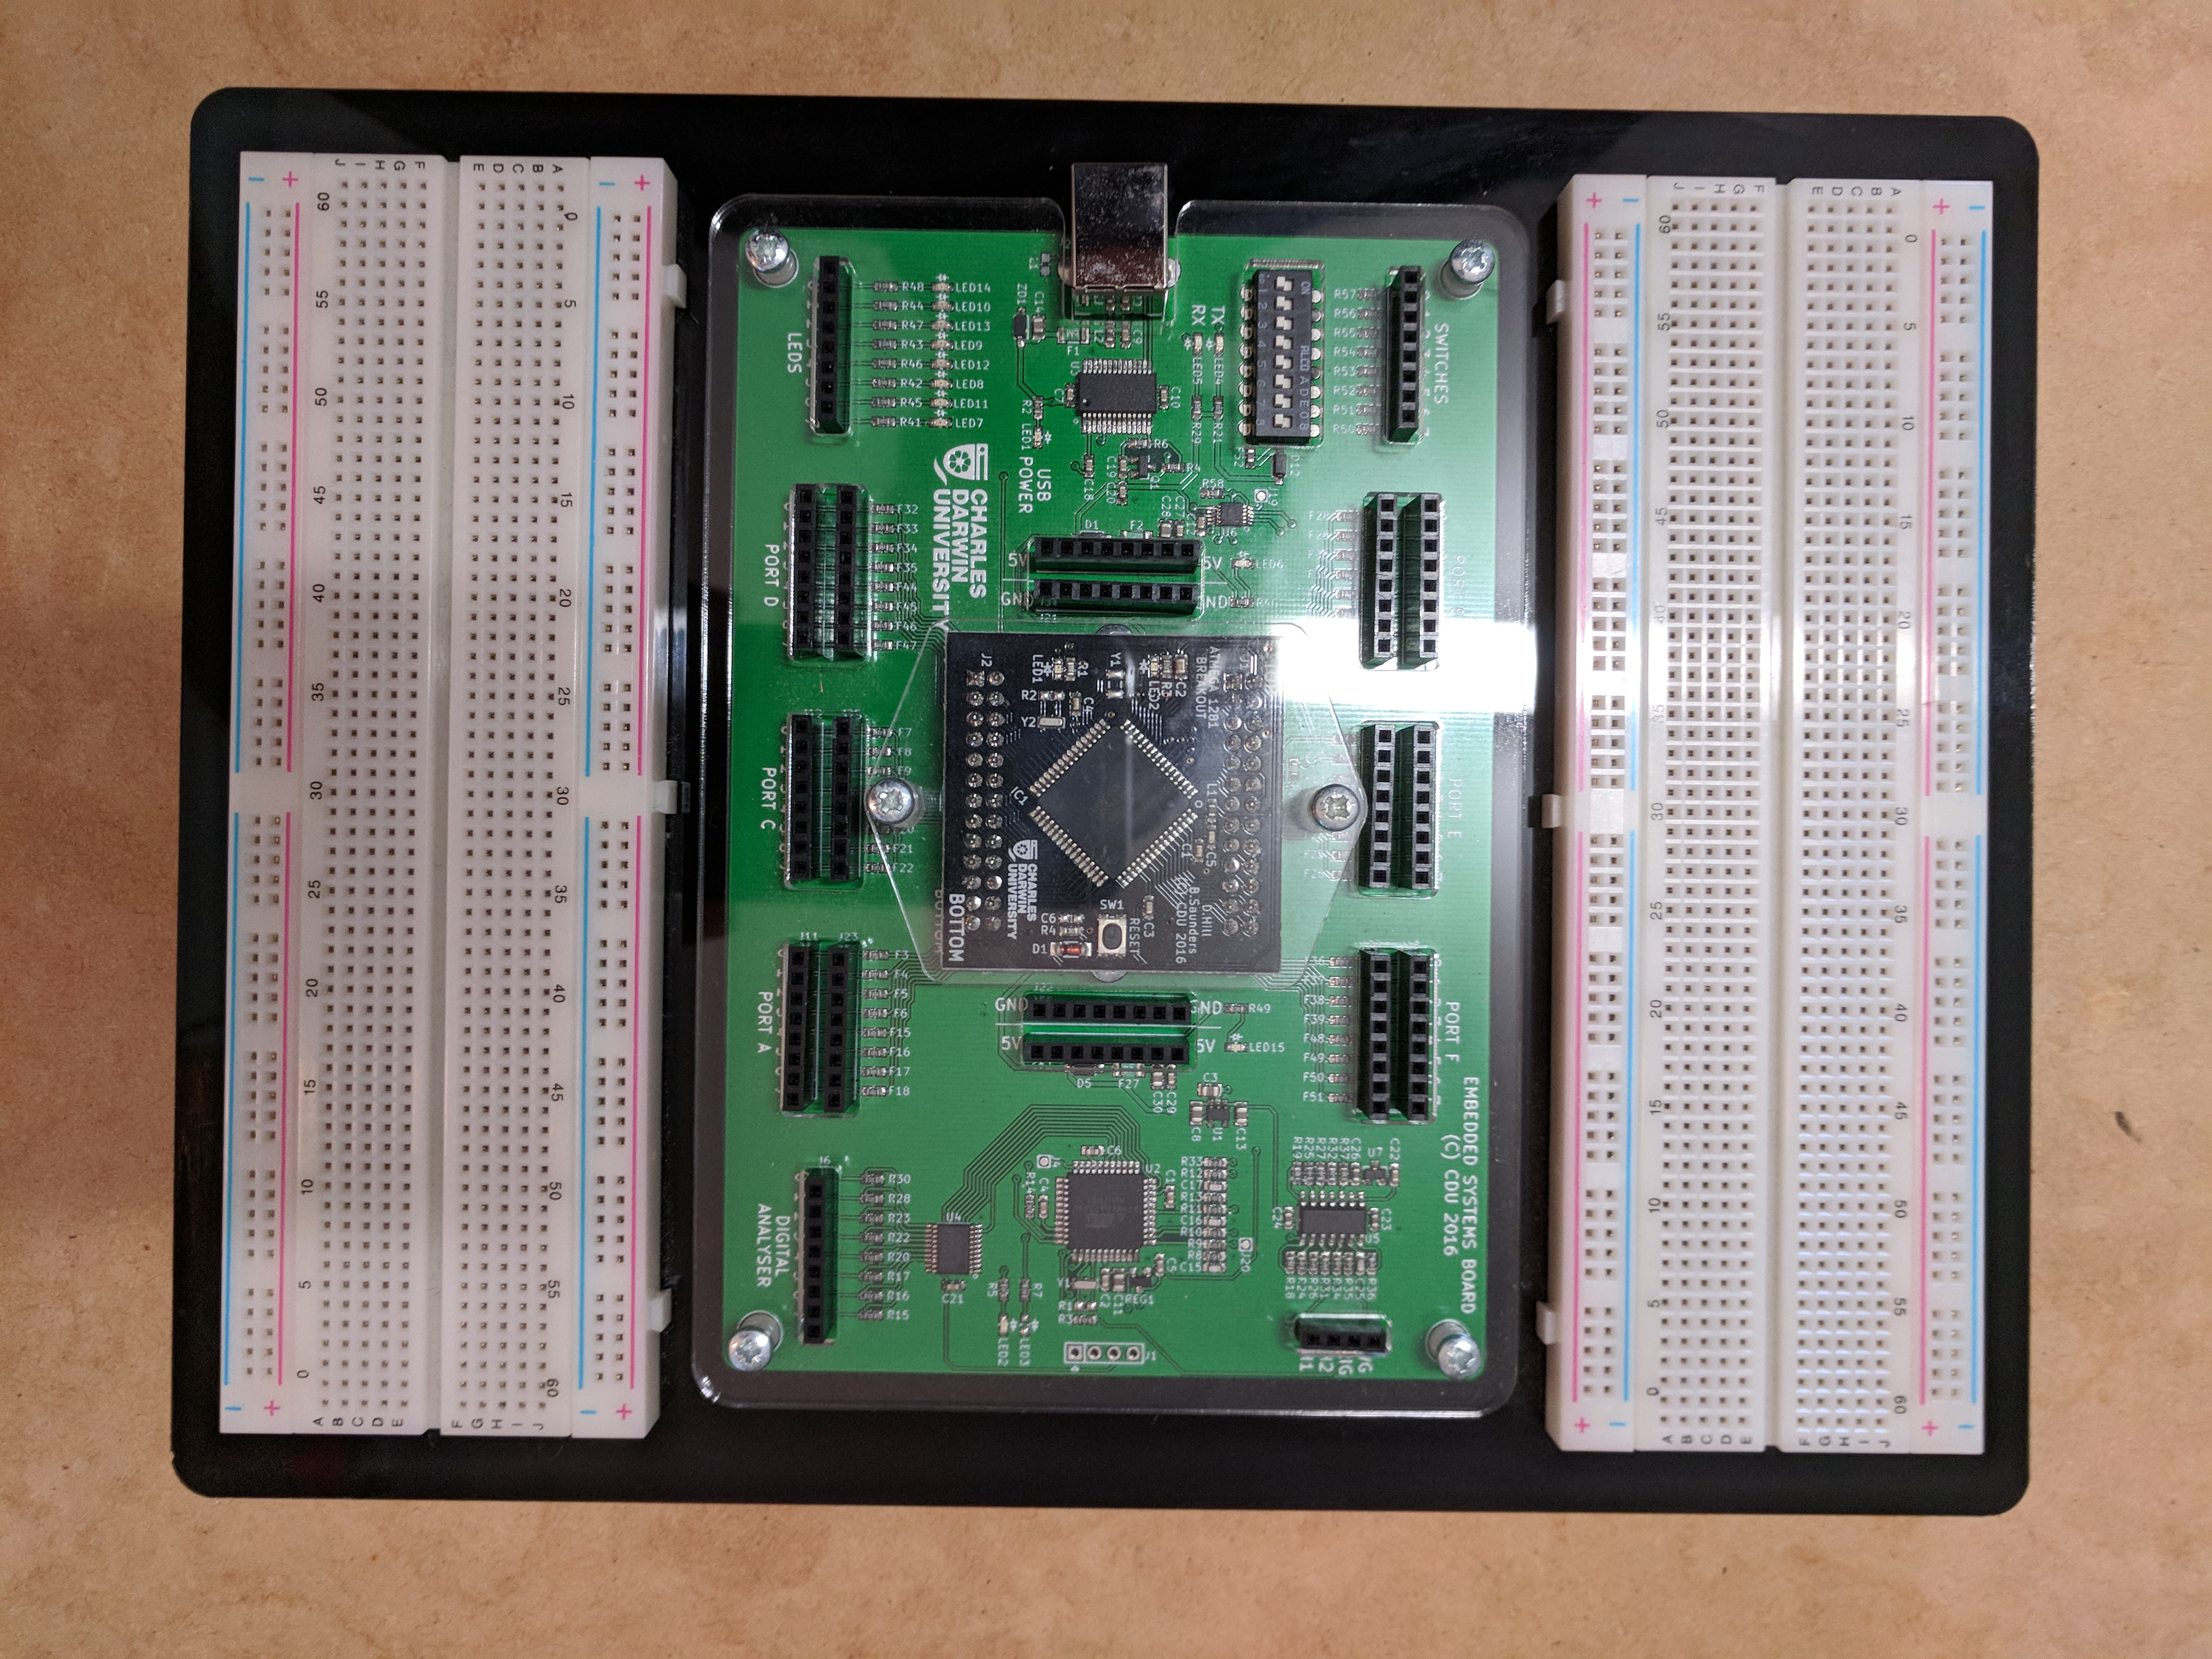
\includegraphics[scale=0.05]{fig1}}
	\caption{The development board which is used in practicals and projects for HIT332: Embedded and Mobile Systems}
\end{figure}

It must be highlighted that these notes have been developed using the board outside of its intended ecosystem. The board is made to be used on CDU's Casuarina Campus in one of the Engineering computer labs. These labs have the appropriate software installed in the correct file paths. These notes have been written using software installed on a personal machine which CDU does not control. Furthermore, the components (other than the development board) used to complete the exercises were sourced independently from a local electronics supplier, independently of CDU. The notes will be highlighted where there has been a significant departure from the intended experience.

\section{Schematic for the Simple Hardware Counter}
This practical involves the creating a simple 4-bit binary counter, using both discrete hardware initially, and then implementing the counter using software. The 74LS193 is an IC which is the core of the 4-bit counter. It must be highlighted that the IC used for this practical was not supplied by CDU, and instead an identical device was acquired from a local electronics store. The IC is driven by a simple clock signal which is produced using software programmed into the ATmega1281 - essentially this will toggle a pin on and off. The schematics for the counter were created in KiCAD following the instructions in the Practical. The completed diagram can be seen in Figure 2.

\begin{figure}[h]
	\centering
	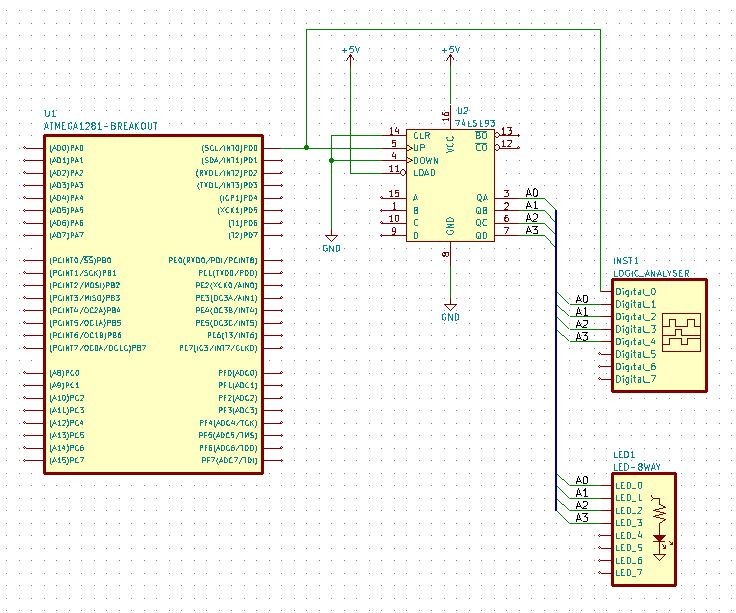
\includegraphics[scale=0.7]{fig2}
	\caption{text}
\end{figure}

\section{Clock Signal Code \& Wiring the Development Board}
A small piece of C code, \verb|main.c|, was developed to generate the clock signal driving the 4-bit counter. This was compiled and loaded into the ATmega1281 with the same makefile process seen in Practical 3. Note that the modified make file, seen in Practical 3, was was copied into the Practical 4 directory. To compile and program the \verb|avr_make all| and the \verb|avr_program PORT=COM3| commands were run from the terminal, respectively. The \verb|main.c| function which provides the clock signal can be seen in Figure 3.


\begin{figure}[h]
	\begin{lstlisting}[style=CStyle]
	#include <avr/io.h>
	#include <util/delay.h>
	
	#define CLOCK_DELAY_MS 16.67
	
	int main (void){
		DDRD = 0x01;     // Set PD0 as output
		while(1){
			PORTD |= (1<<PD0);		// Set PD0 high
			_delay_ms(CLOCK_DELAY_MS);
			PORTD &= ~(1<<PD0);		// Set PD0 low
			_delay_ms(CLOCK_DELAY_MS);
		}
	}
	\end{lstlisting}
	\caption{text}
\end{figure}

Obviously, prior to programming the microcontroller, the development board was wired up according to the schematic shown in Figure 2. The actual physical implementation can be seen in Figure 4.\\

\begin{figure}[h]
	\centering
	\frame{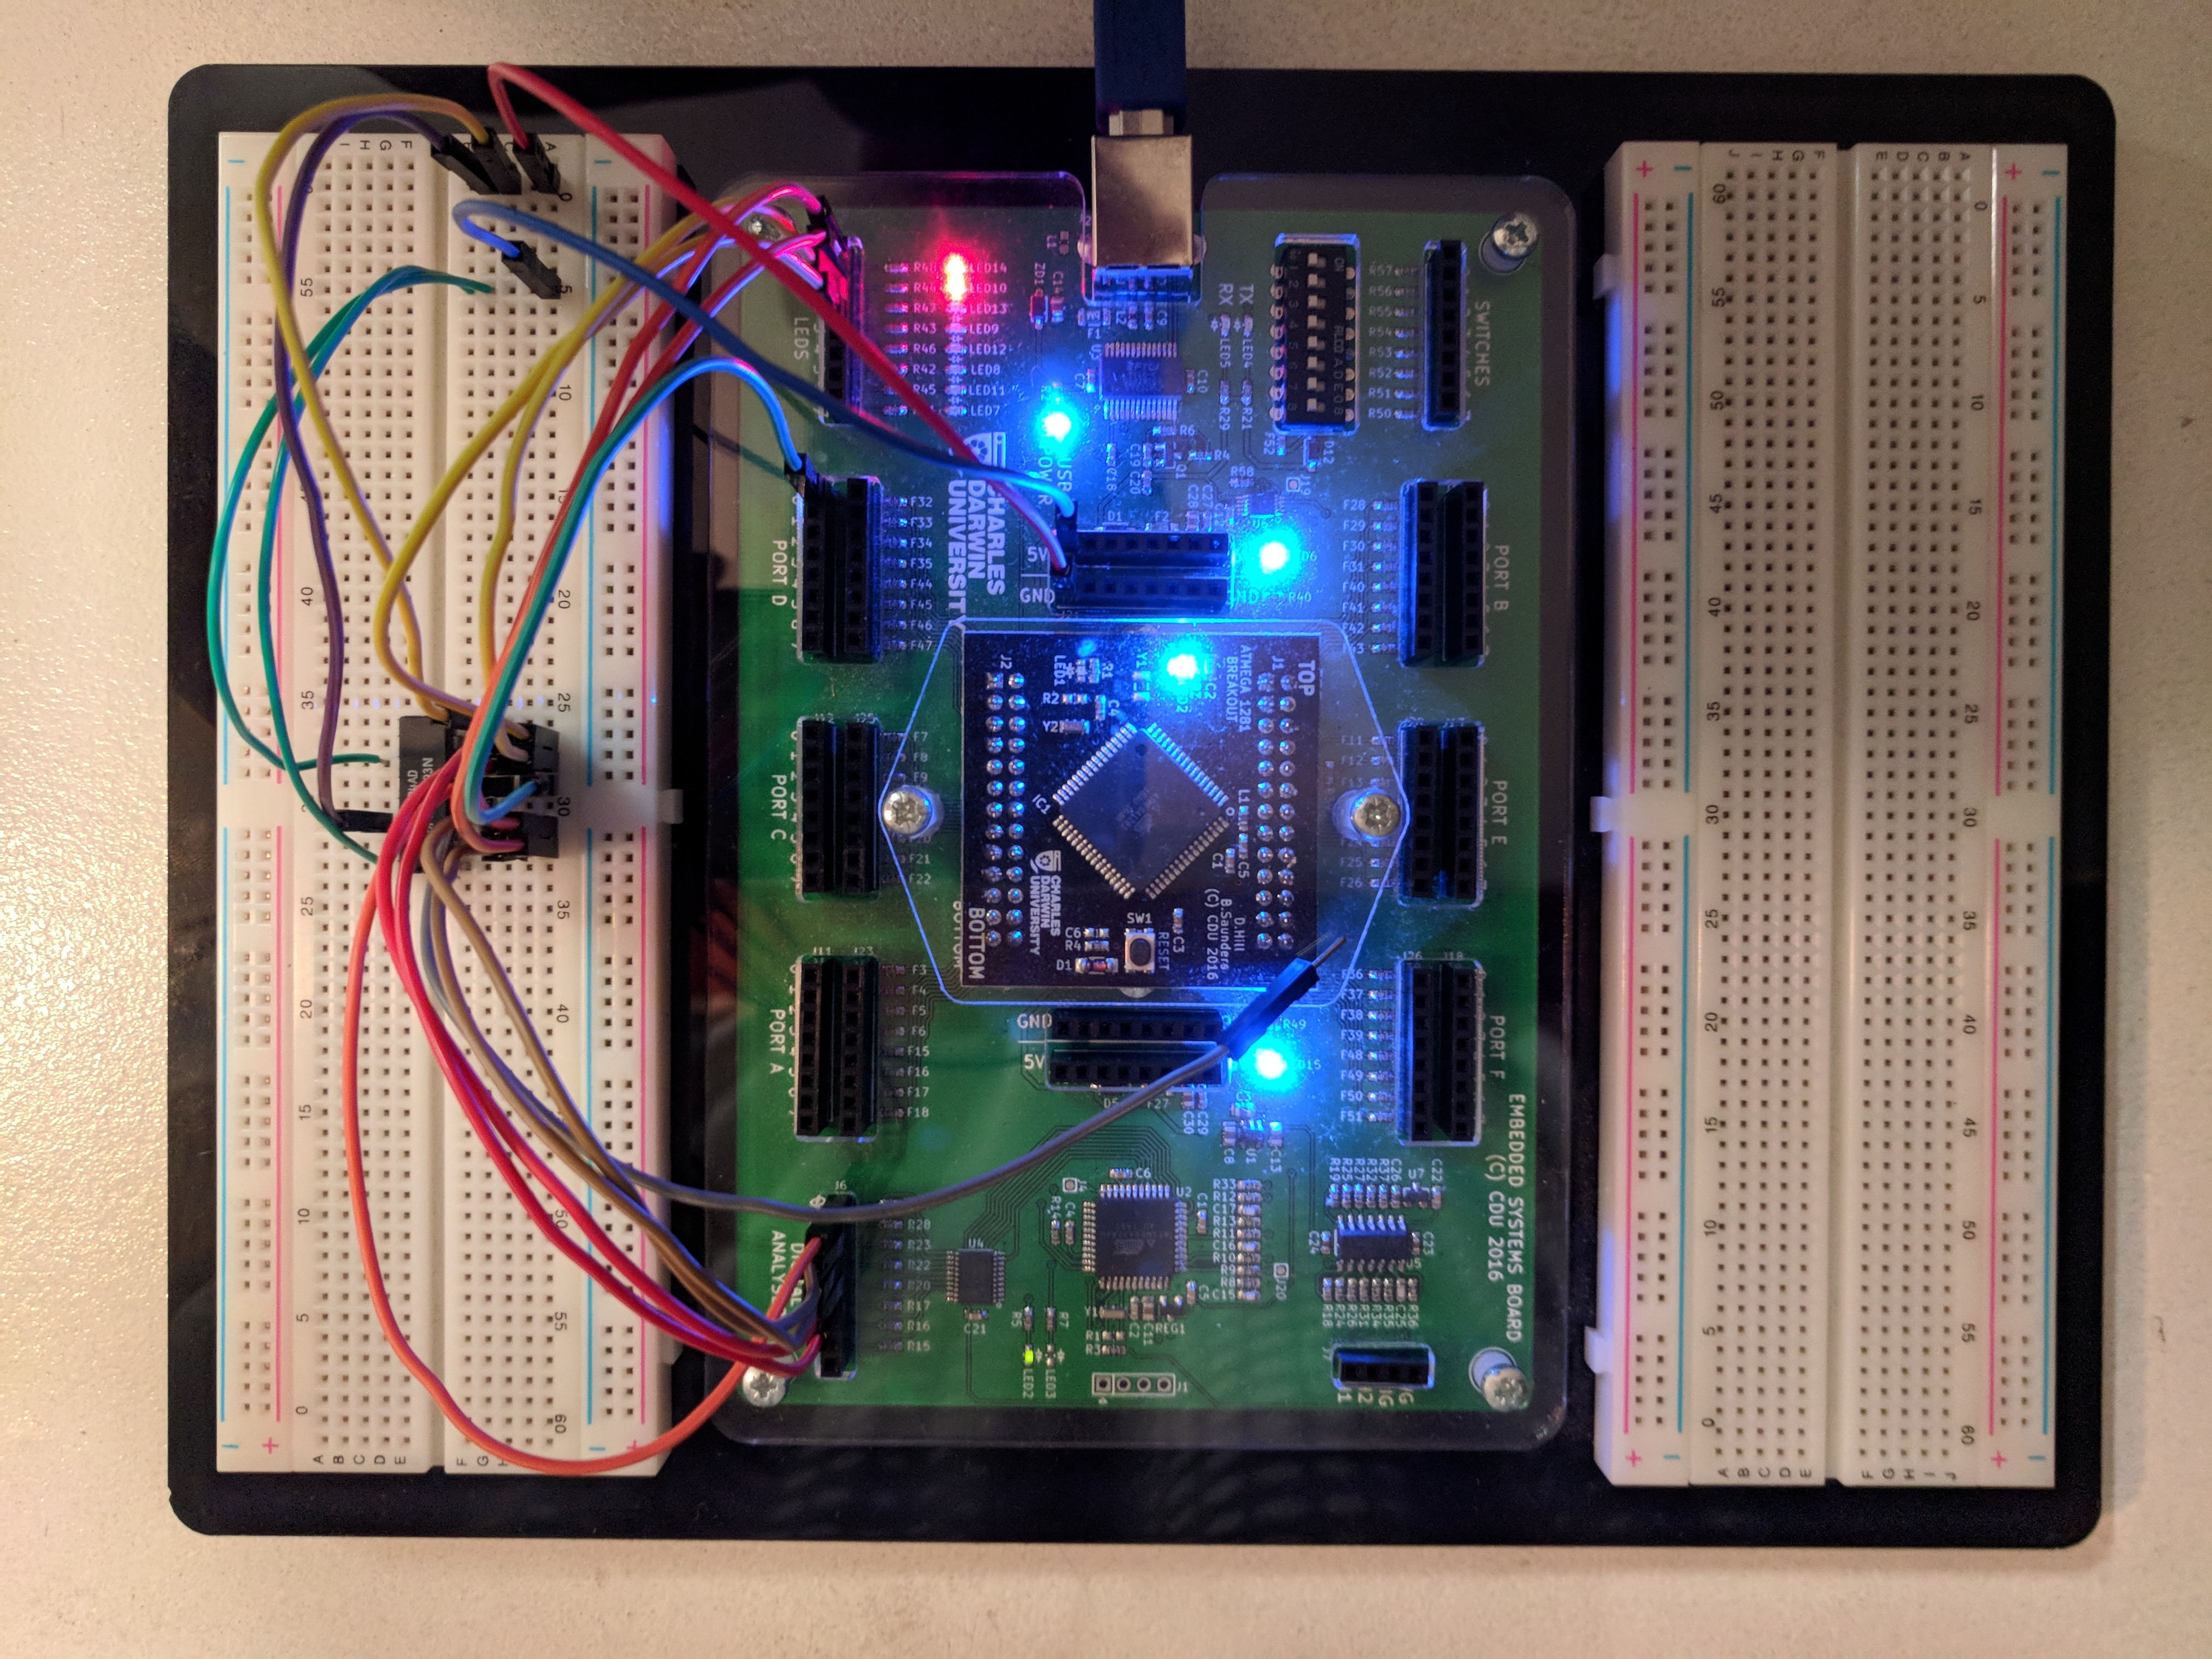
\includegraphics[scale=0.05]{fig4}}
	\caption{text}
\end{figure}

\begin{tcolorbox}
	\textbf{ATTENTION!!}\\
	
	The device did \textbf{not perform as expected}. Initially there was no response from the LED. To troubleshoot this issue, PD0 was connected to a single LED to test that it was toggling correctly - it was. Further testing involved checking the IC was grounded as required. Trial and error, while investigating the correct ground wiring, uncovered correct counter performance. To achieve this pin 4 on the IC needed to be disconnected from the ground. This may be caused by one of 2 possible factors:
	\begin{enumerate}
		\item The IC counter has been incorrectly wired for this practical;
		\item The procured 74LS193 IC differs in some way to the IC which would typically be provided by CDU. 
	\end{enumerate}
\end{tcolorbox}

\section{Using the Logic Counter}
The scope was launched from the CDU Embedded Toolbox. The Digital Analyser was used to visualise the output from the 4-bit counter as per the instructions in the practical. This worked as expected, as shown in Figure 5. Note that the delay in the \verb|main.c| implementation was set to 16.67$\si{\milli\sec}$ which is why the clock signal on channel 0 seems quick.
\begin{figure}[h]
	\centering
	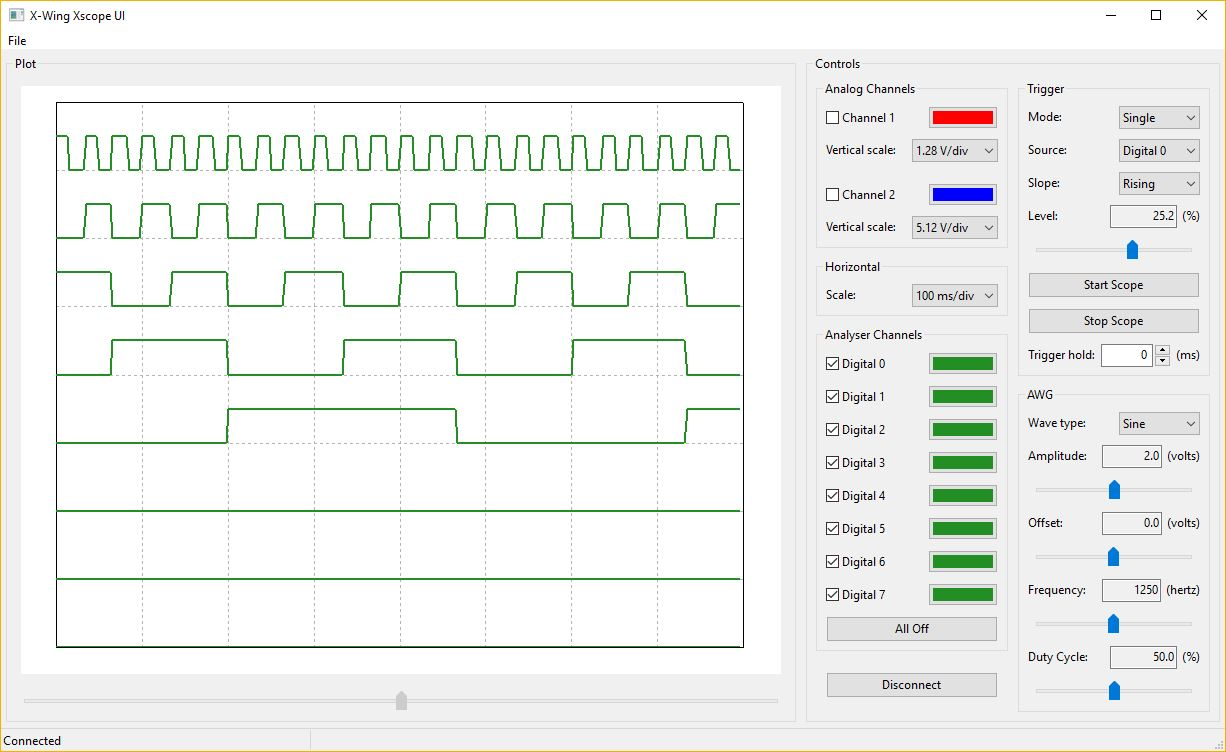
\includegraphics[scale=0.45]{fig5}
	\caption{text}
\end{figure}

\section{Creating a Software Counter}
The final part of this practical sees the recreation of the 4-bit counter using only software. No KiCAD schematics were created for this implementation, however, the physical set up can be seen in Figure 6.

\begin{figure}[h]
	\centering
	\frame{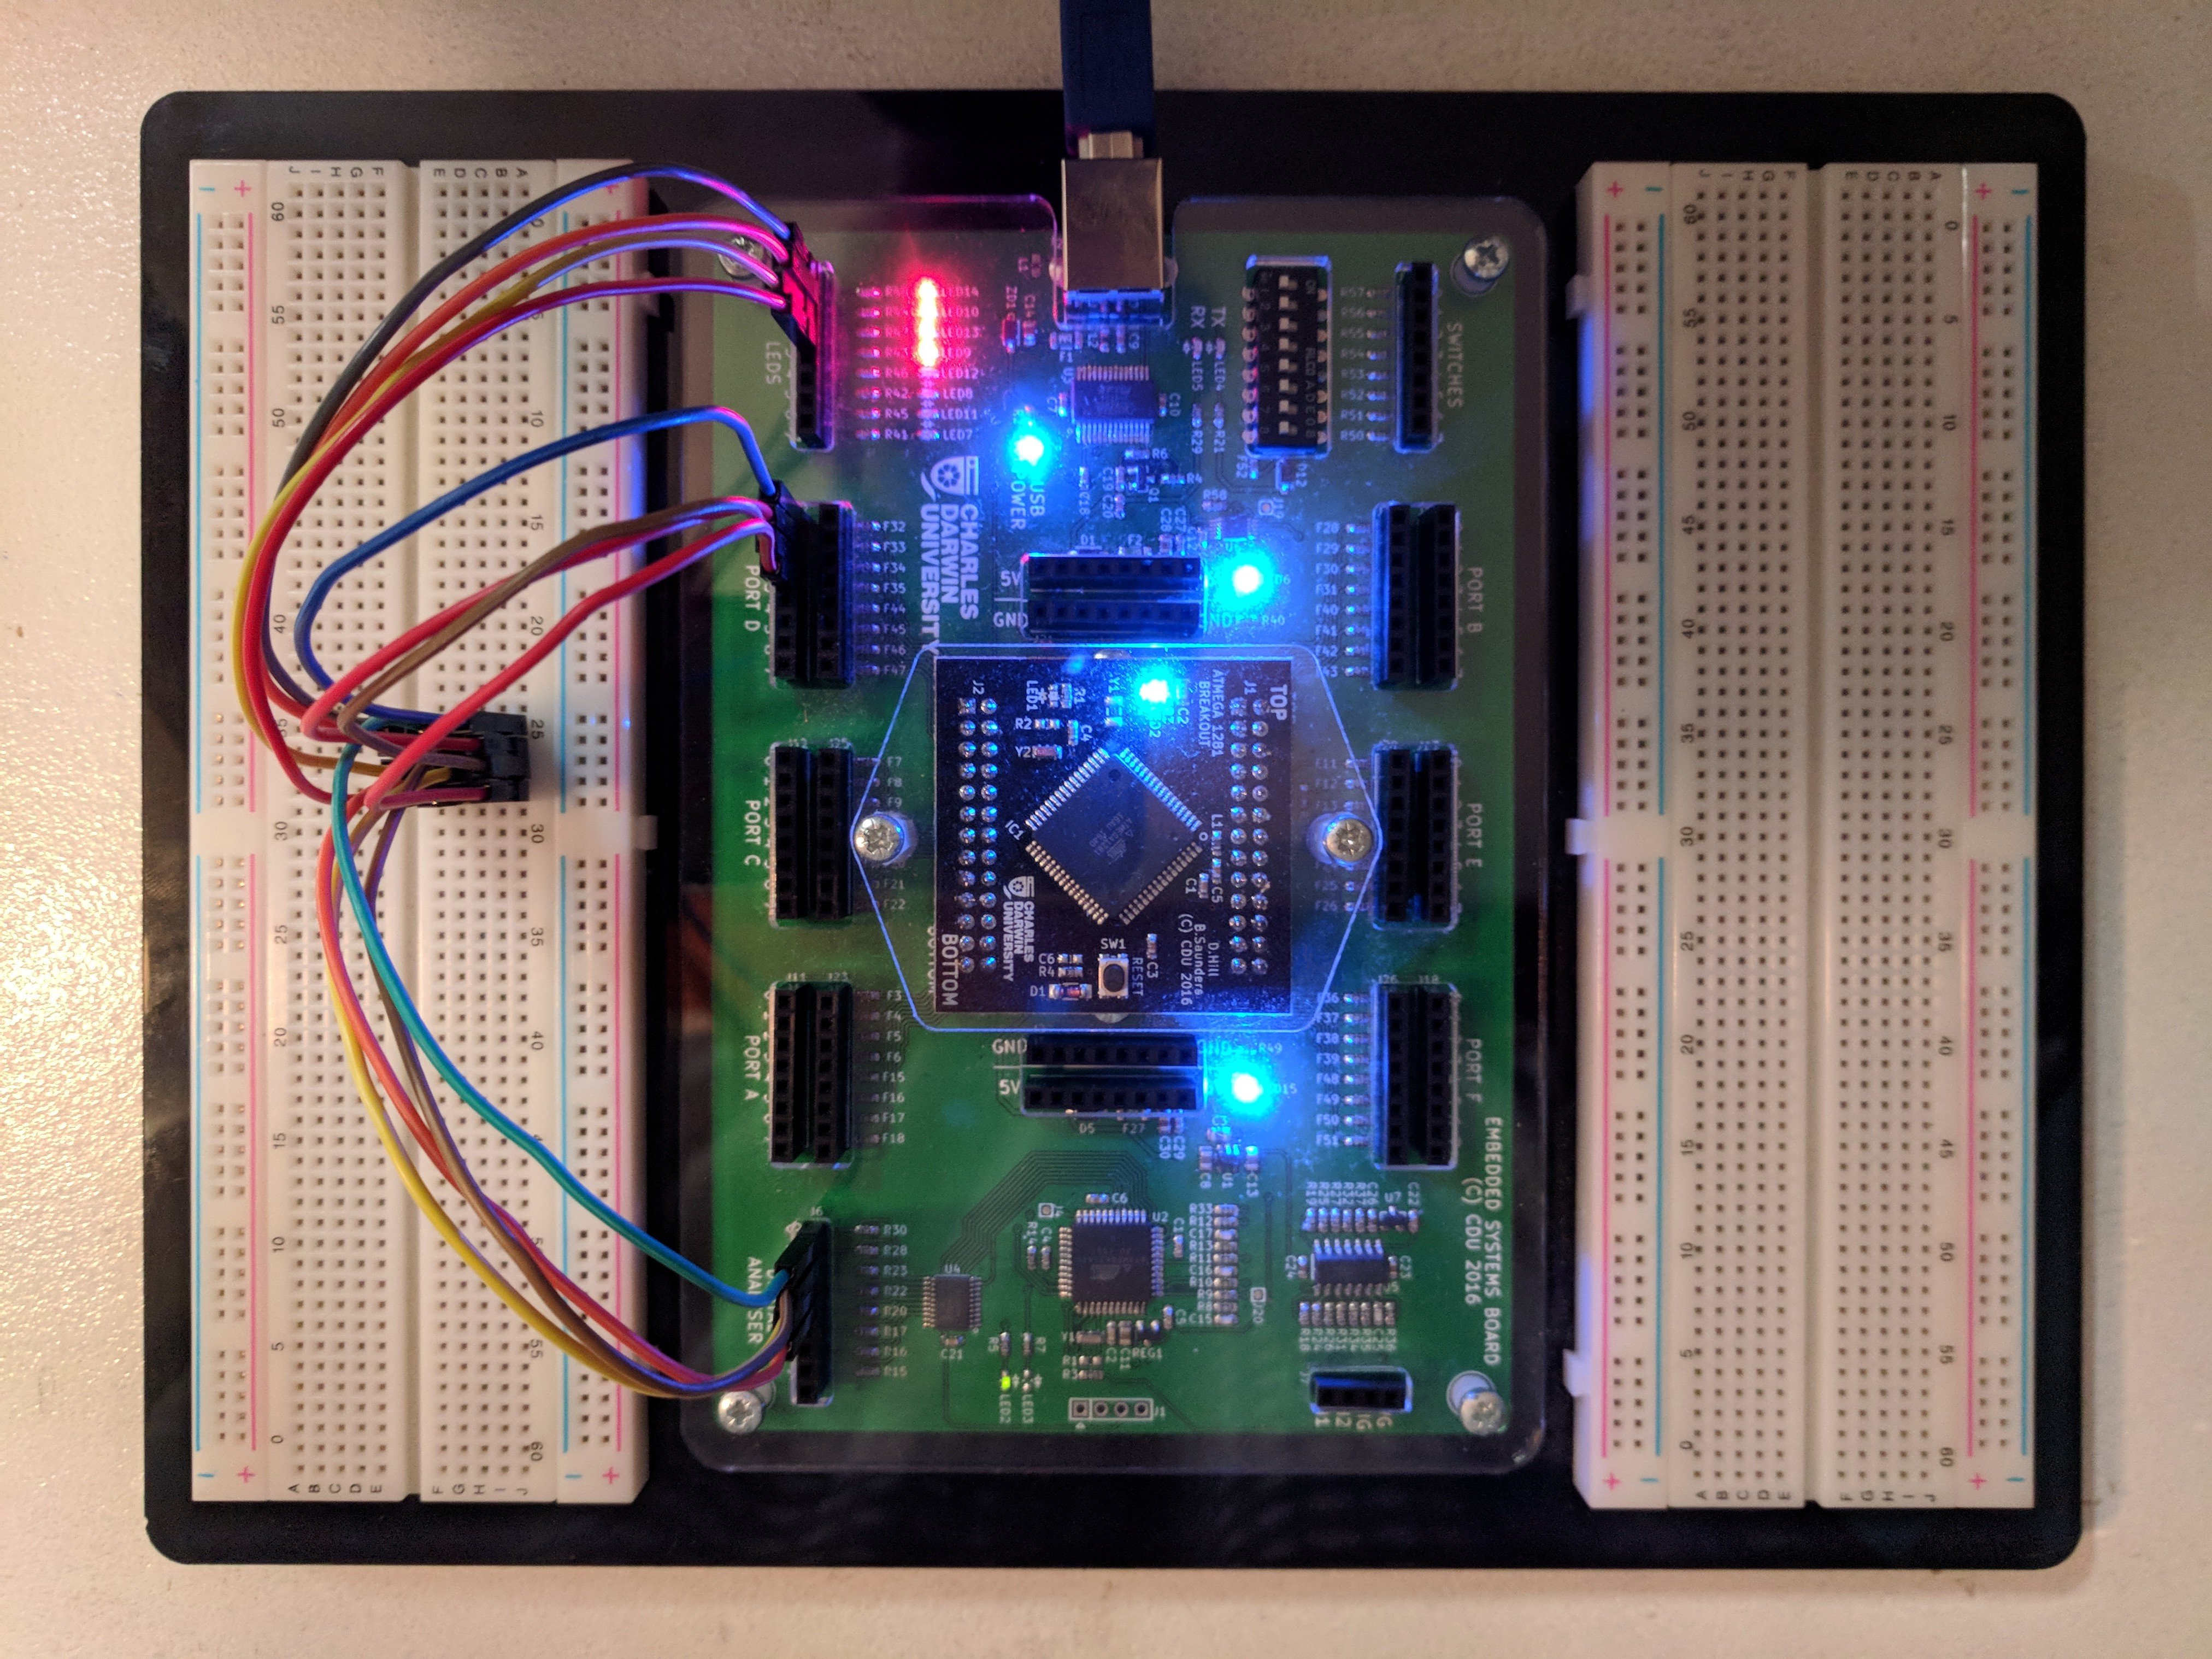
\includegraphics[scale=0.05]{fig7}}
	\caption{text}
\end{figure}

The hardware configuration for this implementation is a simple connection of PD0 to PD3 to LEDs, and the Digital Analyser channels. The C code implementation can be seen in Figure 7. Finally, the Digital Analyser output can be seen in Figure 8.
\begin{figure}[h]
	\begin{lstlisting}[style=CStyle]
	#include <avr/io.h>
	#include <util/delay.h>
	
	#define CLOCK_DELAY_MS 50
	
	int main (void){
	unsigned char counter = 0;
	DDRD = 0x0F;     // Set PD0 to PD3 (inclusive) as output
		while(1){
			counter++;
			if (counter > 15){
				counter = 0;
			}
			PORTD = counter;
			_delay_ms(2*CLOCK_DELAY_MS);
		}
	}
	\end{lstlisting}
	\caption{text}
\end{figure}

\begin{figure}[h]
	\centering
	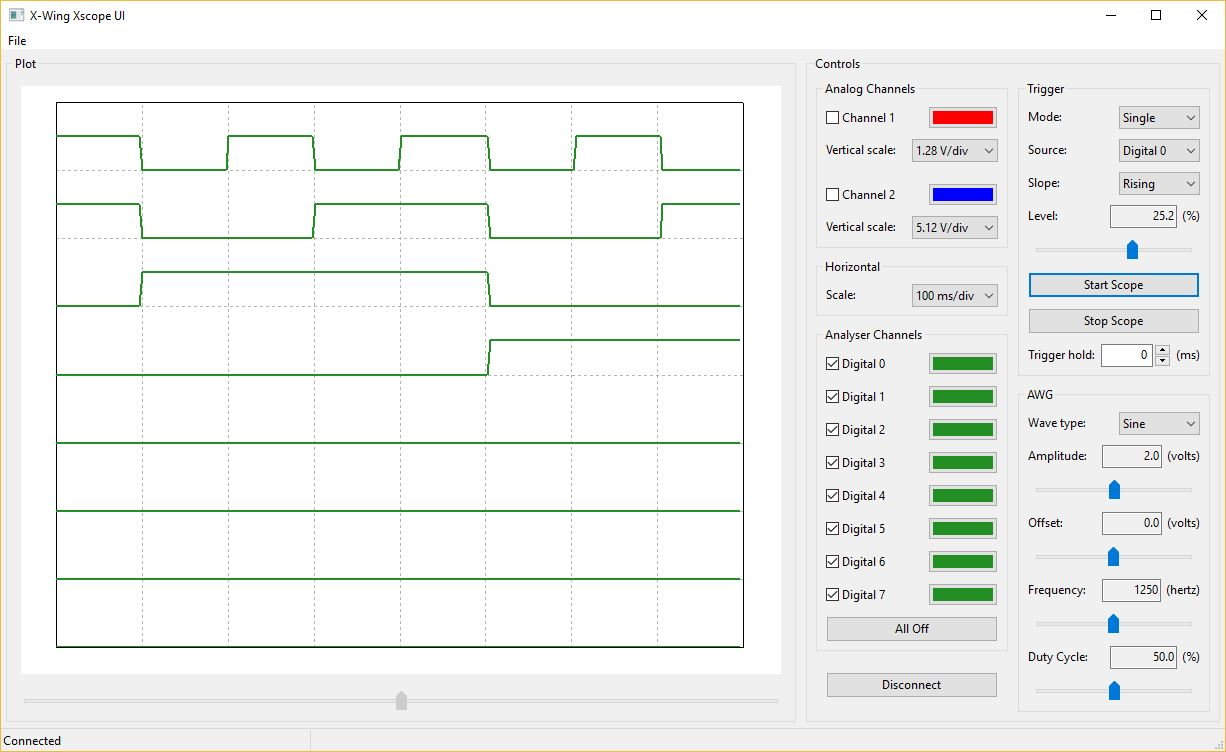
\includegraphics[scale=0.45]{fig6}
	\caption{text}
\end{figure}

\end{document}